\documentclass[tikz,border=8pt]{standalone}
\usepackage{amsmath,amssymb}
\usetikzlibrary{arrows.meta,calc,decorations.markings}

\begin{document}
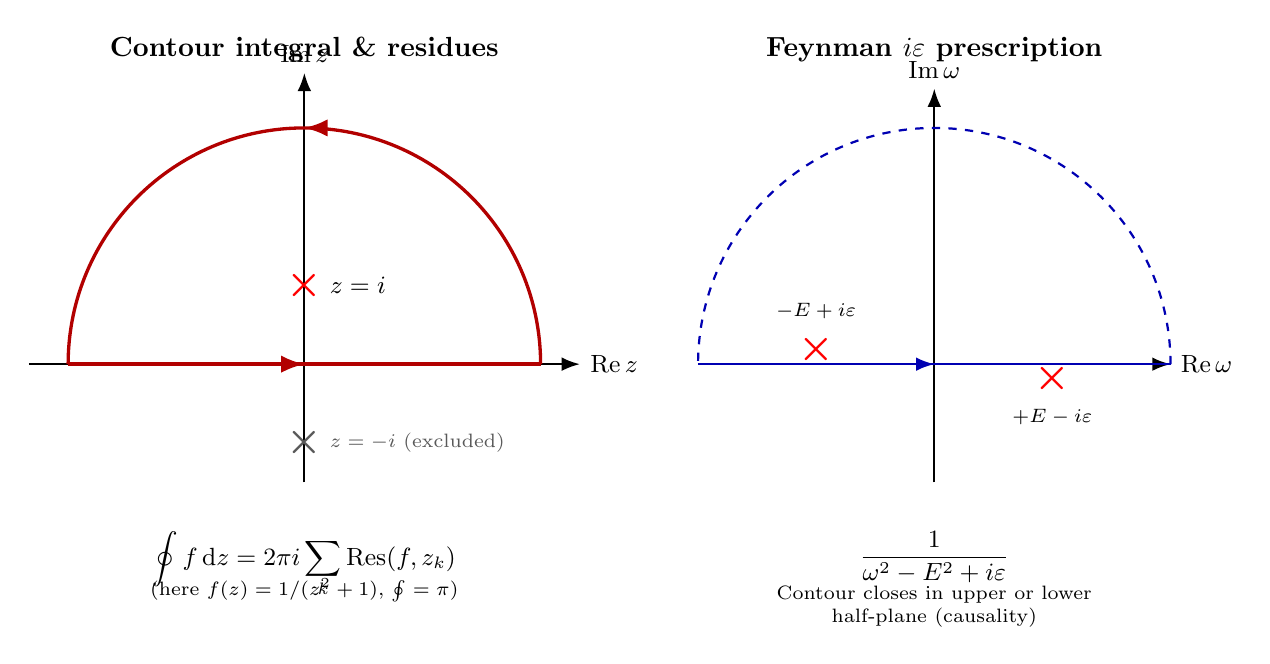
\begin{tikzpicture}[>=Latex]

  % LEFT: closed contour with poles
  \begin{scope}[xshift=0cm]
    \node[font=\bfseries] at (0, 4.0) {Contour integral \& residues};

    \draw[->, thick] (-3.5, 0) -- (3.5, 0) node[right, font=\small]{$\mathrm{Re}\,z$};
    \draw[->, thick] (0, -1.5) -- (0, 3.7) node[above, font=\small]{$\mathrm{Im}\,z$};

    \draw[very thick, red!70!black, postaction={decorate, decoration={markings,
      mark=at position 0.5 with {\arrow{>}}}}] (-3, 0) -- (3, 0);

    \draw[very thick, red!70!black, postaction={decorate, decoration={markings,
      mark=at position 0.5 with {\arrow{>}}}}] (3, 0) arc (0:180:3);

    % poles drawn as ×
    \node[red, font=\Large] at (0, 1.0) {$\boldsymbol\times$};
    \node[font=\small, anchor=west] at (0.20, 1.0) {$z=i$};

    \node[gray!70!black, font=\Large] at (0, -1.0) {$\boldsymbol\times$};
    \node[font=\scriptsize, anchor=west, gray!70!black] at (0.20, -1.0) {$z=-i$ (excluded)};

    \node[font=\small, anchor=north] at (0, -2.0) {$\displaystyle\oint f\,\mathrm dz = 2\pi i\sum_k\mathrm{Res}(f, z_k)$};
    \node[font=\scriptsize, anchor=north] at (0, -2.6) {(here $f(z)=1/(z^2+1)$, $\oint=\pi$)};
  \end{scope}

  % RIGHT: Feynman iε prescription
  \begin{scope}[xshift=8cm]
    \node[font=\bfseries] at (0, 4.0) {Feynman $i\varepsilon$ prescription};

    \draw[->, thick] (-3, 0) -- (3, 0) node[right, font=\small]{$\mathrm{Re}\,\omega$};
    \draw[->, thick] (0, -1.5) -- (0, 3.5) node[above, font=\small]{$\mathrm{Im}\,\omega$};

    \node[red, font=\Large] at (-1.5, 0.18) {$\boldsymbol\times$};
    \node[font=\scriptsize, anchor=south] at (-1.5, 0.45) {$-E + i\varepsilon$};

    \node[red, font=\Large] at (1.5, -0.18) {$\boldsymbol\times$};
    \node[font=\scriptsize, anchor=north] at (1.5, -0.45) {$+E - i\varepsilon$};

    % Closing contour direction (illustrative)
    \draw[thick, blue!70!black, postaction={decorate, decoration={markings,
      mark=at position 0.5 with {\arrow{>}}}}] (-3, 0) -- (3, 0);
    \draw[thick, blue!70!black, dashed] (3, 0) arc (0:180:3);

    \node[font=\small, anchor=north, align=center] at (0, -2.0)
      {$\dfrac{1}{\omega^2 - E^2 + i\varepsilon}$};
    \node[font=\scriptsize, anchor=north, align=center] at (0, -2.7)
      {Contour closes in upper or lower\\half-plane (causality)};
  \end{scope}
\end{tikzpicture}
\end{document}
